\section{The Dataset}\label{sec:dataset}
\subsection{Data Generation}


\subsection{Data Scaling and Transformations}
We shall briefly discuss how the training data is transformed before training.
The targets in the dataset of NLO cross sections can span several orders of magnitude. For practical training of BNNs, this would require
model parameters that also span several orders of magnitude. The result will usually be overflow and thus unsucessful training of the models.
Therefore, we have chosen to map the targets using the base-10 logarithm, i.e $y \mapsto \log_{10}(y)$. More generally, we could choose any base-$a$ logarithm. A practical consideration here is that once the model is trained, any prediction it produces must be transformed back using
the inverse mapping. As we increase the value of $a$, the precision the model can predict decreases. Thus a small error in log-space 
can result in a large error in what we may refer to as target space the larger the value of $a$ is. 


\section{Performance Metrics}\label{seq:perf_metrics}
In this section, we will discuss the performance metrics used to benchmark and measure the performance of the models trained in this thesis.
Due to the inherent probabilistic nature of the models trained, any output the model produces will be a distribution from which we can calculate
a sample mean and variance.

\subsection{Relative Error}
The first and simplest form of performance metric we can use is the \textit{relative error} which is defined as
\begin{equation}
    \epsilon(x^*) = \frac{y_\text{true}- \hat{y}_\text{mean}(x^*)}{y_\text{true}},
\end{equation}
where $y_\text{true}$ is the true target and $\hat{y}_\text{mean}(x^*)$ is the sample mean of the empirical predicitive distribution of the model.

\subsection{Standardized Residuals}
A particularly useful way to represent how well a probabilitic model performs is to study its \textit{standardized residual} which is given by
\begin{equation}
    z(x^*) = \frac{y_\text{true} - \hat{y}_\text{mean}(x^*)}{\hat{\sigma}(x^*)},
\end{equation}
where $\hat{\sigma}(x^*)$ is the square-root of the sample variance. The mathematical representation of the targets $y$ is that they can be decomposed as
\begin{equation}
    y = f(x) + \delta,
\end{equation}
for some true function $f(x)$ and a random noise $\delta \sim \mathcal{N}(0, 1)$, i.e it is distributed according to a standard Normal distribution. But in the case of data produced by \texttt{Prospino}, the noise is neglible which means that $y \approx f(x)$. The regression error obtained through the sample variance is therefore dominated by the predictive distribution computed by the model itself. A good model 



\section{Results}\label{sec:results}
\subsection{Computational Performance}

\subsubsection{CPU versus GPU Performance}
In figure \ref{fig:relative_performance}, we demonstrate the significant speedup that can be achieved
with GPU accelerated sampling when using {\tt TensorFlow Probability} and its implementation of samplers. Here we have used HMC and a fixed $L = 512$ Leapfrog steps.
The speedup itself is due to the utilization of XLA (Accelerated Linear Algebra) which is a highly optimized
linear algebra execution engine \cite{xla}. The time measurements per sample was in the order of magnitude of seconds for the most complex models
tested. An important aspect for practical utilization of BNNs will be ease of training and accelerated sampling with NUTS or HMC, which is automatically achieved if the system can detect an NVIDIA GPU. Moreover, the full training time can be estimated by a few preliminary runs where execution time per sample is measured. This analysis is slightly more difficult when using NUTS. One can however set a maximum tree depth generated with {\tt BuildTree} which is also the case with the implementation employed by {\tt TensorFlow Probability}. As we argued in chapter \ref{chap:no_u_turn_sampler}, the additional computational cost added by NUTS per Leapfrog step is neglible given a sufficiently complex model and/or large dataset.
Thus one can simply perform the measurements using the implementation of HMC and estimate an upper-bound on the computational time defined by the setting of the maximum tree depth.

\begin{figure}
    \centering
    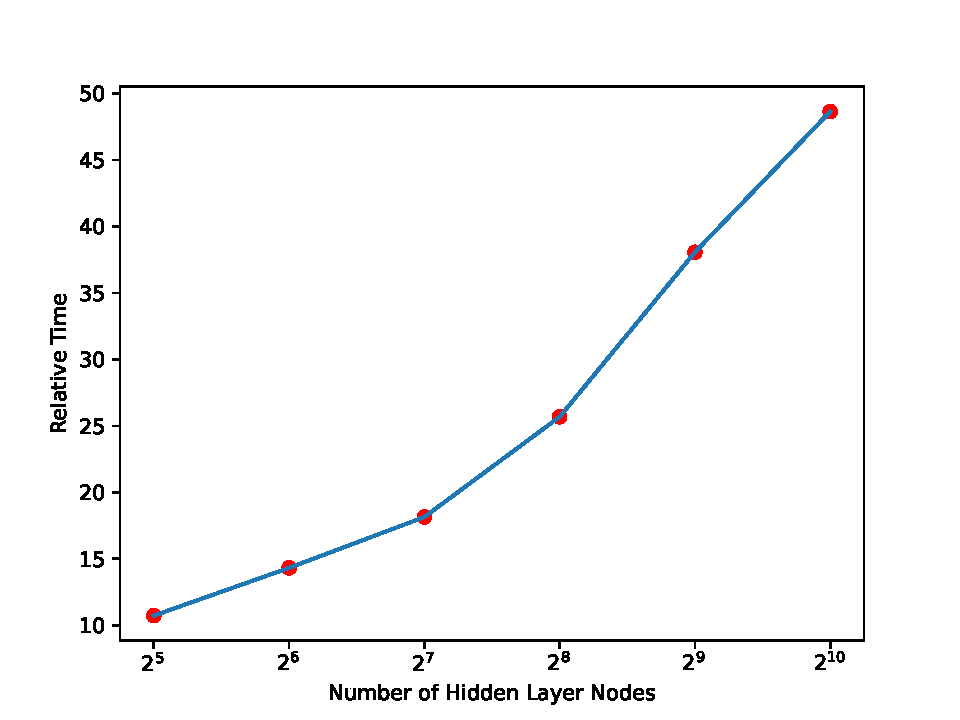
\includegraphics[scale=1]{figures/cpu_vs_gpu/cpu_vs_gpu_performance.pdf}
    \caption{The figure shows the relative measured execution time used per sample using $L = 512$ Leapfrog steps,
    as a function of number of parameters. The CPU measurements are done using an 8-core M1 CPU (Apple Silicon). The GPU measurements
    are made with an NVIDIA Tesla P100 GPU.
    }
    \label{fig:relative_performance}
\end{figure}

\subsubsection{Prediction Time}
As we discussed in the introduction, the execution time's order of magnitude when using {\tt Prospino} is the order of hours. For BNN to be a viable alternative, it must at least significantly reduce the time to compute predictions. In figure \ref{fig:prediction_time}, we 
show the average execution time to compute predictions. For each model, we have sampled 1000 random points and measured the execution time of computing a prediction. The models used are the ones listed in table \ref{tab:deep_models}. Both the sample mean of the predictions and the sample error is computed during the measurement. The measurements were performed on an M1 Apple Silicon CPU using {\tt perf\_counter} from the module {\tt time} provided by the standard library of Python. The order of magnitude is in milliseconds which is a significant speedup over the ones that can be achived with {\tt Prospino}. The BNNs can thus provide a significant reduction in time to predict cross sections but it remains to be seen if the predictions themselves are reliable enough to serve as a viable substitute for {\tt Prospino} calculations which is what we will turn our attention to next.

\begin{figure}
    \centering
    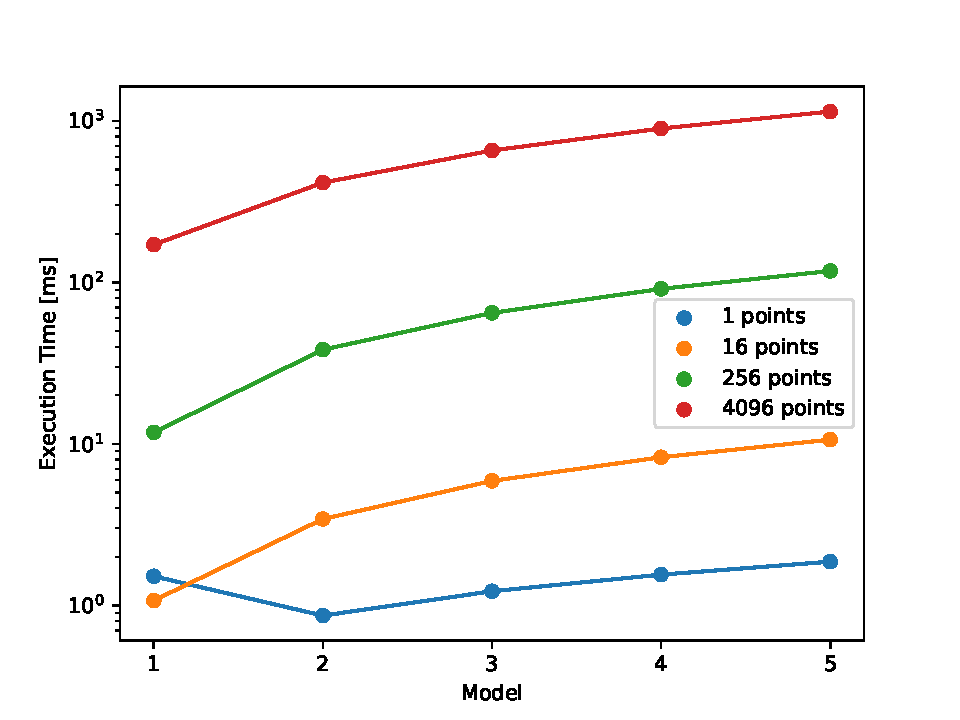
\includegraphics[scale=1]{figures/prediction_time/prediction_time.pdf}
    \caption{The figure shows the average prediction time to compute a prediction given a single input $x$ using the models in table \ref{tab:deep_models}. The average time used is measured in ms and is averaged over 1000 randomly sampled points. The measured time includes computation of the sample mean and sample error.
    }
    \label{fig:prediction_time}
\end{figure}

\subsection{Posterior Distribution of Weights}
An important problem to consider is if we can even justify the use of Monte Carlo samplers to sample from the exact posterior instead of using the approximation employed by variational inference with a parameterized surrogate posterior which is the most ubiquitous method of training BNNs in the literature. The surrogate distribution is usually a factorized normal distribution of the form
\begin{equation}
    q \propto \prod_{i, j, \ell} \mathcal{N}(\mu_{ij}^\ell, (\sigma_{ij}^\ell)^2),
\end{equation}
meaning for each parameter in the model, we assume its posterior distribution can be written as an independent Gaussian distribution with a mean $\mu_{jk}^\ell$ and a standard deviation $\sigma_{ij}^\ell$. The method sports some fairly obvious advantages like the fact that one can perform \textit{online training}, i.e. continue training once new data becomes available starting from an earlier \textit{checkpoint} by using $q$ obtained during earlier training as the prior. The way we have trained BNNs in this thesis does not permit this form of training because we cannot formulate a prior based on the empirical distribution we have sampled. Thus we cannot use the weights of the model that we have already sampled to continue training. We must start over entirely and discard the empirical distribution we obtained with the prior dataset. 

It has been widely discussed that BNN posteriors are typically found to be multi-modal \cite{google_bnn_posteriors}. We demonstrate this observation in figure \ref{fig:}


\begin{figure}
    \centering
    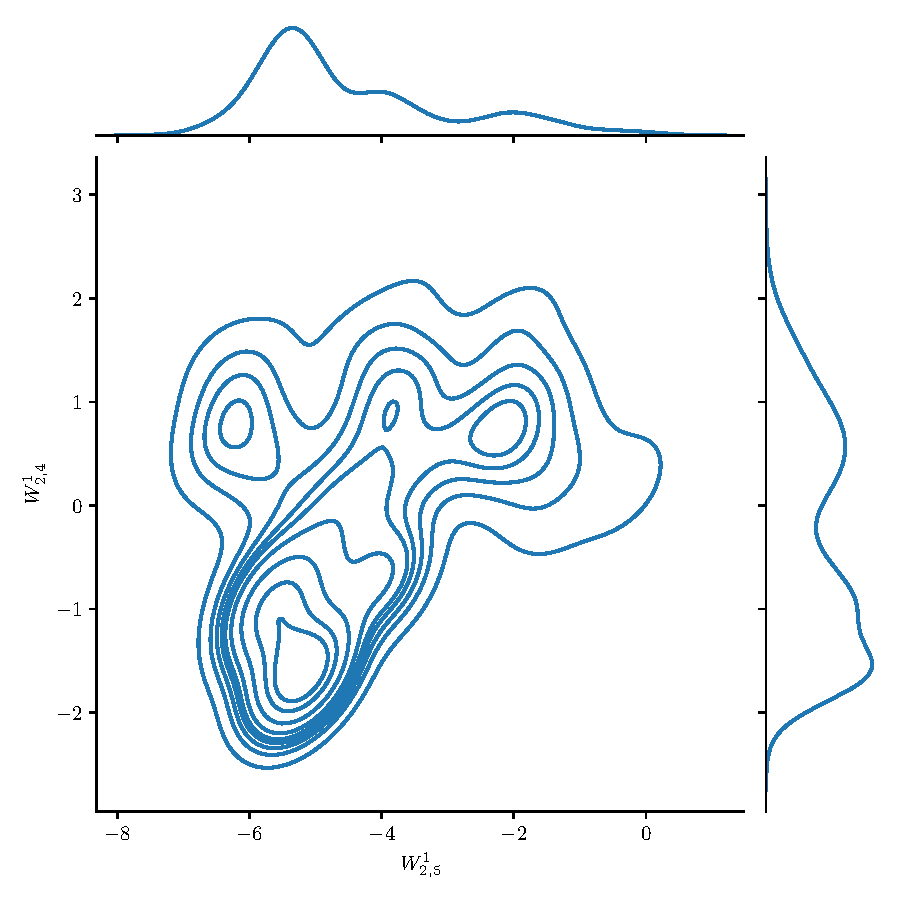
\includegraphics[scale=0.5]{figures/posterior_distribution/posterior_weights1.pdf}
    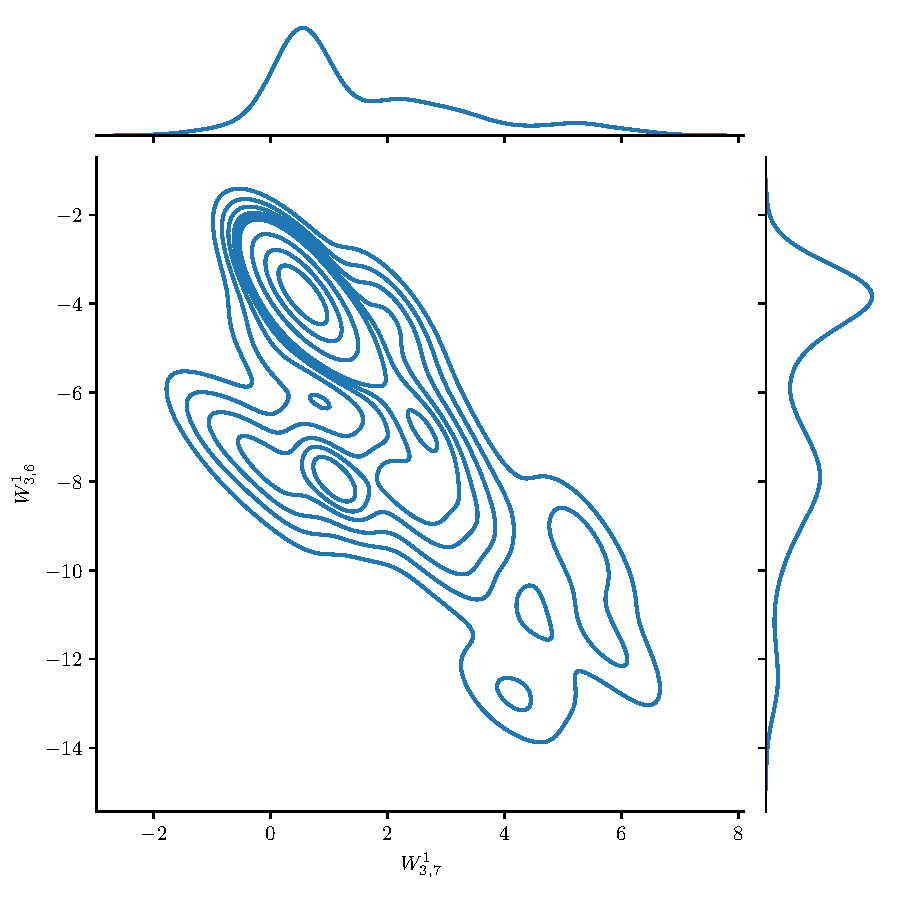
\includegraphics[scale=0.5]{figures/posterior_distribution/posterior_weights2.pdf}
    \caption{The figure shows the projection of the empirical distribution onto the planes spanned by $(W_{2,4}^1, W_{2,5}^1)$ on the left and onto the plane spanned by $(W_{3,7}^1, W_{3, 6}^1)$ on the right, using the samples from model 2 in table \ref{tab:deep_models}. The distributions are approximated using kernel density estimation. 
    }
    \label{fig:standardized_residual}
\end{figure}


\subsection{Benchmarks of Hyperparameters}\label{subsec:benchmarks}
\subsubsection{Baseline Model}
\subsubsection{Pretraining}
\subsubsection{Burn-in length}
\subsubsection{Number of model parameters}

\subsection{Neutralino-Neutralino Cross Sections}\label{subsec:neuralino_experiments}

\begin{table}[h!]
    \centering
\begin{tabular}{c@{\hspace{1cm}}c@{\hspace{1cm}}c@{\hspace{1cm}}c@{\hspace{1cm}}c@{\hspace{1cm}}c}
\hline
    Burn-in steps & \makecell{Number \\of \\steps between} & Kernel & \makecell{Number \\ of \\ results} & \makecell{Pretraining \\ epochs} & \makecell{Pretraining \\ batch size} \\
\hline
    2500 & 10 & NUTS & 1000 & 1000 & 32 \\
\hline
\end{tabular}
\caption{
    The table shows the training configuration used to sample the models listed in table~\ref{tab:deep_models}.
}
\label{tab:NN_mse_scores}
\end{table}


\begin{table}[h!]
    \centering
\begin{tabular}{c@{\hspace{1cm}}c@{\hspace{1cm}} c}
\hline
      Model number & Architechture & Number of parameters \\
\hline
    1 & 5-50-1 & 351\\
    2 & 5-50-50-1 & 2901\\
    3 & 5-50-50-50-1 & 5451\\
    4 & 5-50-50-50-50-1 & 8001\\
    5 & 5-50-50-50-50-50-1 & 10551\\
\hline
\end{tabular}
\caption{
    The table shows the models used in this section. For each model, 1000 sampled networks are used to
    generate each result shown in this section. The architecture describe number of nodes per layer.
    For each hidden layer, the same activation function is used. The final layer uses an identity function.
}
\label{tab:deep_models}
\end{table}

\begin{figure}
    \centering
    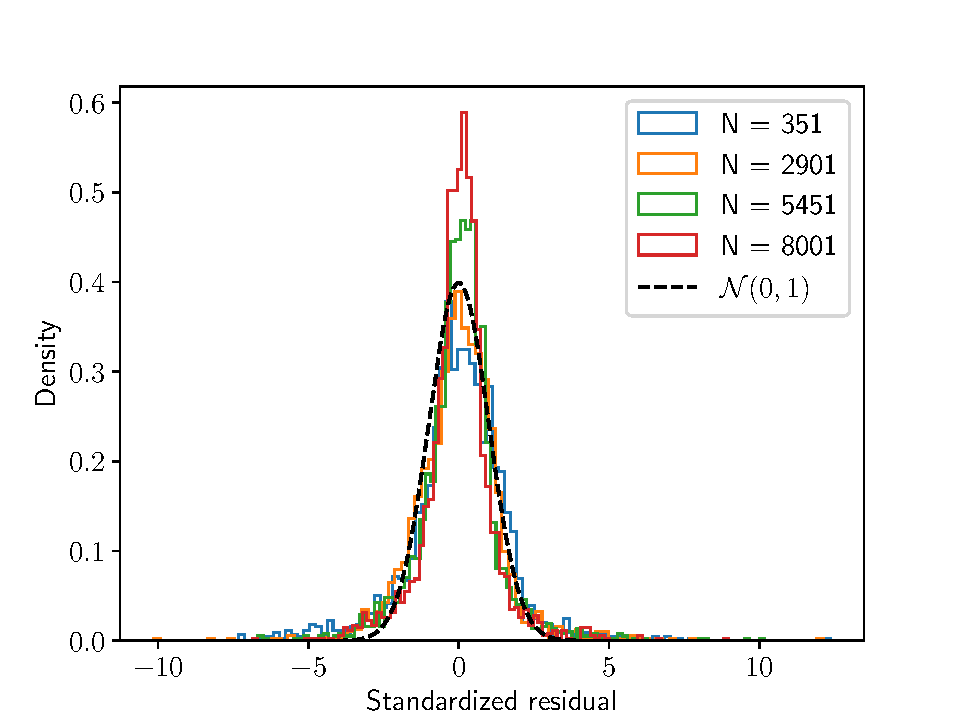
\includegraphics[scale=1]{figures/standardized_residuals/standardized_residual_simple_models.pdf}
    \caption{The figure shows histograms of the standardized residuals computed for 
        different BNNs. The normal distribution is drawn as dotted line. 
    }
    \label{fig:standardized_residual}
\end{figure}

